\documentclass[11pt]{article}
\usepackage[a4paper,margin=2.5cm]{geometry}
\usepackage{newtxtext,newtxmath}
\usepackage[T1]{fontenc}
\usepackage{graphicx}
\usepackage{booktabs}
\usepackage{multirow}
\usepackage{amsmath}
\usepackage[numbers,sort&compress]{natbib}
\usepackage{xcolor}
\usepackage[colorlinks=true,linkcolor=black,citecolor=blue!50!black,urlcolor=blue!50!black]{hyperref}
\usepackage{caption}
\captionsetup{font=small,labelfont=bf}
\usepackage{xurl}
\usepackage{enumitem}
\setlist{itemsep=1pt,topsep=3pt}
\newcommand{\yn}{Yunmo-Next-1B}

\title{\textbf{Yunmo-Next-1B: A Traditional-Chinese-First\\Hybrid Linear-Attention Language Model\\Trained on a Single Consumer GPU}}
\author{YuhuanStudio\\[2pt]\small\url{https://github.com/YuhuanStudio/Yunmo-Next}}
\date{Technical report, November 2026}

\begin{document}
\maketitle

\begin{abstract}
We present \yn{}, a 1.008B-parameter language model for Traditional Chinese, English, code and mathematics,
trained from scratch on 19.76B tokens with about $1.05\times10^{20}$ FLOPs, mostly on one 12\,GB RTX 4070 Ti.
The model stacks 15 four-layer cells of one gated grouped-query attention layer and three Kimi Delta Attention
layers, reads every sublayer input through low-rank block attention residuals, and was grown in depth from 24
to 60 layers during pretraining. We describe the architecture and the paired experiments behind each choice,
a 65,536-entry two-phase BPE tokenizer whose corpus is sized by target token exposure, the training route and
the memory techniques that fit it on the consumer GPU, instruction tuning, and CUDA-graph decoding.
In evaluation, the model trails 2026 open models of similar size, trained on up to about 1,400 times more tokens,
on English and knowledge benchmarks, and is at chance on letter-scored MMLU and TMMLU+. At equal pretraining
compute it is ahead of every Pythia checkpoint and an OLMo~2 checkpoint on eight English tasks, and between
the annealed 300M and 530M DataDecide models, whose compute brackets its own. On Traditional Chinese Wikipedia articles
written after every compared model's training data it has lower bits per byte than six other open-weight
models, including 2B models, also on articles with no overlap with its training data; on three non-Wikipedia
Traditional Chinese corpora it is on par with the strongest 1B models rather than ahead. We release the base and
instruction-tuned weights, quantized versions with measured quality and speed, the tokenizer, training and
evaluation code, and all evaluation outputs under Apache-2.0.
\end{abstract}

\section{Introduction}

Small open language models are usually built by organizations that can spend $10^{22}$--$10^{24}$ FLOPs on
them. This report documents a model built under a different constraint: one consumer GPU with 12\,GB of memory,
supplemented by 230 rented GPU-hours, and a total pretraining budget of about $10^{20}$ FLOPs. The model is
Traditional-Chinese-first: most of its Chinese training text is in Traditional script, and its tokenizer was
built for it.

The constraint shaped every decision. Attention with a growing key--value cache is limited to 15 of 60 layers,
10 of them with a sliding window; the other 45 are Kimi Delta Attention (KDA) layers with a fixed-size
state~\cite{kimilinear2025}. The model was grown from 24 to 60 layers in three steps so that early training ran
on a smaller network. Optimizer state is kept in BF16 with Kahan-compensated momentum instead of FP32 master
weights. These choices let the 60-layer model train at 16K context on the 12\,GB card.

Our contributions are:
\begin{itemize}
\item A hybrid KDA/GQA architecture with \emph{low-rank block attention residuals}, a \emph{Cell-Echo} routing
  bias and \emph{cell-phase} feed-forward widths that keep tensor shapes valid under depth growth
  (\S\ref{sec:arch}), each chosen with paired training runs.
\item A tokenizer whose corpus is sized by target token exposure and whose vocabulary is built in two phases,
  with cross-boundary ``superwords'' (\S\ref{sec:tok}).
\item A documented route for pretraining a 1B model on a single consumer GPU: depth growth, precision and memory
  techniques, and their cost (\S\ref{sec:train}).
\item An evaluation that separates the effect of compute from the recipe (equal-compute comparisons with Pythia,
  DataDecide and OLMo~2), measures knowledge with continuous metrics where accuracy is at chance, and tests a
  Traditional Chinese result for training-data overlap and for domain (\S\ref{sec:eval}).
\item Weights, quantized versions in five formats with measured quality and speed, code and all evaluation
  outputs.
\end{itemize}

The model's main weakness is knowledge: at this compute, letter-scored knowledge benchmarks are at chance and
the instruction-tuned model trails 2026 models of similar size on every chat benchmark. We report this in the
same detail as the results that favor the model.

\section{Architecture}\label{sec:arch}

\begin{figure}[!t]
  \centering
  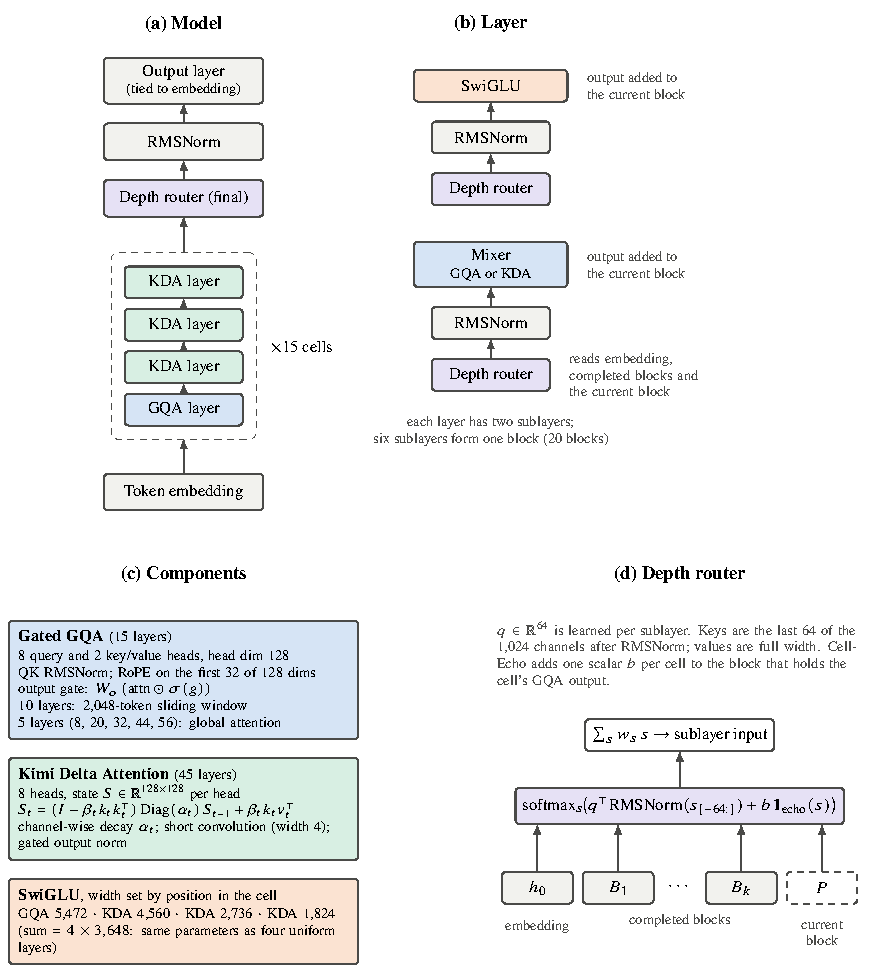
\includegraphics[width=0.8\textwidth]{../figures/architecture_2x2.pdf}
  \caption{Architecture. (a) 15 cells of one GQA layer and three KDA layers; a final depth router feeds the
  output norm and the tied output layer. (b) Each layer has two sublayers, each reading its input through a
  depth router and an RMSNorm; six sublayers form one block. (c) Layer components. (d) The depth router
  attends over the embedding, the completed blocks and the running sum of the current block.}
  \label{fig:arch}
\end{figure}

\yn{} is a 60-layer decoder of width 1,024 built from a repeating four-layer cell: one gated GQA
layer~\cite{gqa2023,gatedattn2025} followed by three KDA layers (Figure~\ref{fig:arch}). Table~\ref{tab:spec}
lists the configuration.

\begin{table}[t]
\centering\small
\caption{Model configuration.}\label{tab:spec}
\begin{tabular}{@{}lp{0.78\textwidth}@{}}
\toprule
Parameters & 1,008,058,231 (embedding tied to the output layer) \\
Layers & 60 = 15 cells of [GQA, KDA, KDA, KDA] \\
GQA & 8 query / 2 KV heads of dim.~128; QK RMSNorm; RoPE on 32 of 128 dims ($\theta=10^7$); output gate \\
 & 10 layers with a 2,048-token sliding window; 5 global (layers 8, 20, 32, 44, 56) \\
KDA & 8 heads, key/value dim.~128, state $128\times128$ per head; width-4 short convolution \\
Feed-forward & SwiGLU, width by cell position: 5,472 / 4,560 / 2,736 / 1,824 \\
Depth routing & low-rank block attention residuals (keys: 64 channels), Cell-Echo \\
Vocabulary & 65,536 (256 reserved protocol IDs) \\
Training context & 16,384 tokens \\
\bottomrule
\end{tabular}
\end{table}

\paragraph{Hybrid cell.} GQA layers normalize queries and keys per head, apply rotary
embedding~\cite{rope2021} to the first 32 of 128 dimensions, and gate the attention output elementwise,
$W_o(\mathrm{attn}\odot\sigma(g))$~\cite{gatedattn2025}. KDA layers use the gated delta rule with channel-wise
decay of Kimi Linear~\cite{kimilinear2025,gateddeltanet2024,deltanet2024},
\begin{equation}
S_t = \left(I-\beta_t k_t k_t^{\top}\right)\mathrm{Diag}(\alpha_t)\,S_{t-1} + \beta_t k_t v_t^{\top},
\qquad o_t = S_t^{\top} q_t,
\end{equation}
through the flash-linear-attention kernels~\cite{fla2024}. Only the 5 global GQA layers keep a cache that grows
beyond 2,048 positions.

\paragraph{Low-rank block attention residuals.} Following Attention Residuals~\cite{attnres2026}, each sublayer
reads its input through softmax attention over earlier representations instead of a residual sum. Sublayer
outputs are grouped into blocks of six. The sources are the token embedding $h_0$, the summed output of each
completed block $B_1,\dots,B_k$, and the running sum $P$ of the current block. With a learned query
$q\in\mathbb{R}^{64}$ per sublayer,
\begin{equation}
x = \sum_{s} w_s\, s,\qquad w=\mathrm{softmax}_s\!\left(q^{\top}\mathrm{RMSNorm}(s_{[-64:]}) + b\,\mathbf{1}_{\mathrm{echo}}(s)\right),
\end{equation}
where keys use only the last 64 of the 1,024 channels and values are full width. Completed-block logits for all
six reads of a block are computed in one pass and the partial block is merged with an online-softmax update;
source keys are recomputed per block in the backward pass. In a 24-layer test this version reached nearly the
loss of full-rank keys at 0.95$\times$ instead of 0.85$\times$ the throughput of the previous block-skip
residual.

\paragraph{Cell-Echo.} In each cell, the router that feeds the last layer's mixer has one zero-initialized
scalar $b$ added to the logit of the block containing that cell's GQA output (15 scalars in total).

\paragraph{Cell-phase SwiGLU widths.} For cell position $r\in\{0,1,2,3\}$ the SwiGLU~\cite{swiglu2020} width is
\begin{equation}
w_r=\mathrm{round}_{16}\!\left(d\left(1+\tfrac12\cos(\pi r/3)\right)\right),\qquad d=3{,}648,
\end{equation} giving 5,472, 4,560, 2,736 and 1,824. The
widths sum to $4d$, so a cell has the parameters of four uniform layers. Because growth adds whole cells,
every existing layer keeps its position and tensor shapes.

\paragraph{Design experiments.} Each choice was made with short paired runs of a 24-layer model (about 440M
parameters, 4--8M tokens per arm, identical initial weights, one to three seeds). Table~\ref{tab:arch-exp}
summarizes them. These are directional results at small scale; no component was ablated in the 1B model.

\begin{table}[t]
\centering\footnotesize\setlength{\tabcolsep}{4pt}
\caption{Design experiments at 24 layers: difference in final validation loss (candidate minus control,
nats/token; negative favors the candidate), one entry per seed.}\label{tab:arch-exp}
\begin{tabular}{@{}lllr@{}}
\toprule
Choice & Candidate vs.\ control & $\Delta$ loss & Throughput \\
\midrule
KDA heads & 8 heads $\times$ 128 vs.\ 16 $\times$ 128 & $-0.0100$, $-0.0097$ & 1.21$\times$ \\
Attention ratio & 2:1 vs.\ 3:1 KDA:GQA & $+0.0101$ (3:1 kept) & 1.01$\times$ \\
Depth routing & rank-64 block AttnRes vs.\ block-skip residual & $-0.0009$, $-0.0350$, $-0.2106$ & 0.95$\times$ \\
Cell layout & GQA first with Cell-Echo vs.\ GQA last & $-0.0032$, $-0.0081$ & 1.00$\times$ \\
FFN widths & cosine widths vs.\ uniform & $-0.0044$, $-0.0097$ & 1.01$\times$, 0.99$\times$ \\
Lexical memory & removed vs.\ hashed lexical memory & $-0.025$, $-0.030$ & -- \\
\bottomrule
\end{tabular}
\end{table}

\section{Tokenizer}\label{sec:tok}

The tokenizer is a 65,536-entry byte-level BPE (all 256 bytes in the base alphabet), no unknown token, single-digit splitting and
no normalization; IDs 65,280--65,535 are reserved for a chat, reasoning and tool-call protocol. Two decisions
shape it.

\paragraph{Corpus sized by token exposure.} The tokenizer corpus is sized so that each domain's share of
training \emph{tokens} matches its planned share of model training. With target share $q_d$ and a reference
tokenizer producing $\tau_d$ tokens per byte in domain $d$, the byte budget is
$b_d=(q_d/\tau_d)/\sum_j(q_j/\tau_j)$; budgets were recomputed with the new tokenizer until they moved by less
than one percentage point. The corpus is 101,241 documents (200.2\,MB) from 21 source families, with a held-out
set of 10,166 documents fixed before any candidate was scored.

\paragraph{Two-phase vocabulary.} Phase~1 learns 60,280 entries within standard pre-tokenization boundaries.
Phase~2 re-encodes the corpus with the phase-1 tokenizer and learns 5,000 ``superwords'' of up to 8 phase-1
tokens that may cross word and punctuation boundaries (but not digits or line breaks), an independent
implementation of the cross-boundary idea of SuperBPE and BoundlessBPE~\cite{superbpe2025,boundlessbpe2025}.
Both phases are serialized into one standard \texttt{tokenizer.json}.

On the blind held-out set it uses 6.5\% fewer tokens than a phase-1-only control trained on the same data
(English $-12.3\%$, mathematics $-9.9\%$, Chinese prose $-1.3$ to $-1.8\%$), and a 91.9M-parameter model trained
with it at an equal token budget reached 1.9868 against 1.9963 bits per byte (one seed). It failed one
preregistered external gate, a lexicon cost below 2.48 on OpenFormosa's PangolinBench (2.57; control 2.62).

\begin{figure}[t]
  \centering
  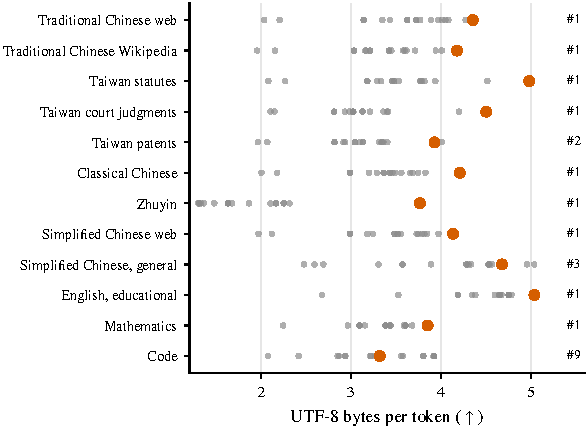
\includegraphics[width=0.62\textwidth]{../figures/tokenizer_compression.pdf}
  \caption{UTF-8 bytes per token of the Yunmo-Next tokenizer (orange) and 17 other tokenizers (grey) on 12
  domains; rank at right. These domains come from source families also used to train the Yunmo-Next tokenizer,
  which favors it.}
  \label{fig:tok}
\end{figure}

Figure~\ref{fig:tok} compares 18 tokenizers on 12 domains drawn from its own source families, which favors it.
On text outside its sources (Chinese Wikipedia articles created after 2026-10-01 and five corpora published by
OpenFormosa~\cite{openformosa}), it needs fewer tokens than OpenFormosa's PangolinTokenizer on all seven sets
(4--31\% more text per token) with 57\% of its vocabulary; the 188K-entry TAIDE tokenizer is ahead on the new
Traditional Chinese Wikipedia text (3.72 vs.\ 3.65 bytes per token).

\section{Pretraining data}\label{sec:data}

The pretraining data combines Traditional Chinese web text (FineWeb2-HQ and a filtered FineWeb2
subset~\cite{fineweb2hq2025}), Chinese web and educational text converted from Simplified script (Ultra-FineWeb,
OpenCSG FineWeb-Edu-Chinese, IndustryCorpus2~\cite{ultrafineweb2025}), Chinese Wikipedia and Wikisource,
Taiwanese government documents, English educational and synthetic text (FineWeb-Edu, Ultra-FineWeb
L3~\cite{fineweb2024,ultrafineweb2025}), mathematics (FineMath~\cite{smollm2}) and code (The Stack, Kaggle
notebooks). Simplified Chinese prose was converted with OpenCC \texttt{s2twp}~\cite{opencc}, protecting code,
URLs and other machine text, and deduplicated again after conversion. Through the 14.4B-token capability stage
the largest families were FineWeb2-HQ (5.11B tokens), Ultra-FineWeb L3 English (2.32B) and code (1.49B). The
final 5.36B tokens came from one 16K pack of 3.38B tokens (58.0\% Chinese, 31.3\% English, 9.7\% code by
document-level identification), seen about 1.59 times. Decontamination was by normalized substring matching
against benchmark inputs; there was no near-duplicate or semantic decontamination across the full corpus. The
training data is not redistributed; the sources and their licenses are listed in the data report.

\section{Training}\label{sec:train}

\begin{table}[t]
\centering\small
\caption{Training route. Held-out bits per byte is measured at 8K context on the same 125 documents from 16
strata at every stage.}\label{tab:route}
\begin{tabular}{@{}lrrrrlr@{}}
\toprule
Stage & Layers & Params & Context & Tokens & GPU & Held-out BPB \\
\midrule
24 layers & 24 & 443.5M & 8K & 2.000B & 4070 Ti & 0.7956 \\
36 layers & 36 & 631.7M & 8K & 2.000B & 4070 Ti & 0.7589 \\
48 layers & 48 & 819.9M & 8K & 2.500B & 5090 & 0.7385 \\
48 layers, long context & 48 & 819.9M & 32K & 0.500B & 5090 & 0.8339 \\
60 layers & 60 & 1,008.1M & 16K & 5.000B & 5090 & 0.7190 \\
60 layers, new mixture & 60 & 1,008.1M & 16K & 2.400B & 5090 $\rightarrow$ 4070 Ti & 0.7160 \\
Extension & 60 & 1,008.1M & 16K & 4.161B & 4070 Ti & 0.6860 \\
Anneal (released) & 60 & 1,008.1M & 16K & 1.200B & 4070 Ti & 0.6706 \\
\bottomrule
\end{tabular}
\end{table}

\paragraph{Route and depth growth.} Table~\ref{tab:route} lists the stages and Figure~\ref{fig:train} the
held-out loss. Growth from $L$ to $L+12$ layers copies all existing layers, their routers and optimizer state,
and appends 12 layers initialized from the first three cells (for 48$\rightarrow$60, source layers
$[0,\dots,47]+[0,\dots,11]$); the cell layout keeps every tensor shape valid~\cite{stacking2024}. The
36$\rightarrow$48 step changed held-out BPB by $+0.06\%$ immediately after mapping. A 0.5B-token stage at 32K
context raised short-context held-out BPB by 12.9\% without producing durable long-context ability; the
following 60-layer stage recovered it. We did not compare growth with training a 60-layer model from scratch.

\begin{figure}[t]
  \centering
  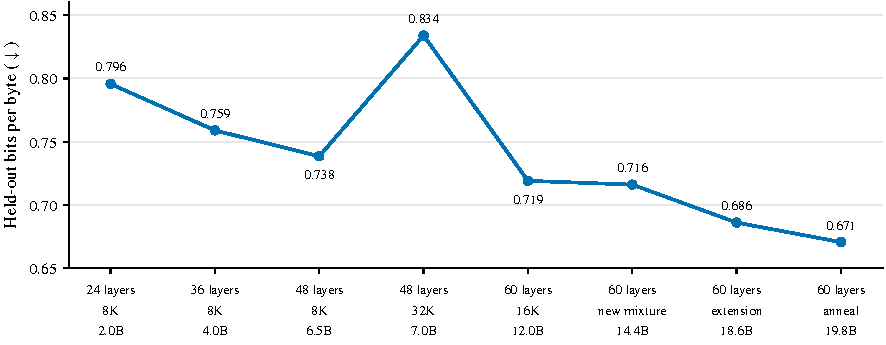
\includegraphics[width=\textwidth]{../figures/training_curve.pdf}
  \caption{Held-out bits per byte (125 documents, 8K context) at the end of each stage, with cumulative
  training tokens.}
  \label{fig:train}
\end{figure}

\paragraph{Objective and batch.} Next-token cross-entropy on packed rows with document isolation (attention
masks, KDA state and positions reset at every boundary, cross-document targets masked). Every update is
65,536 tokens; at 24 layers early in training, 4$\times$ and 16$\times$ larger updates gained under 5\%
throughput and reached worse validation loss at an equal token budget.

\paragraph{Optimizer.} Matrices use Muon~\cite{muon2024,muonscalable2025} with three role-specific variants:
U-NorMuon~\cite{normuon2025} for the SwiGLU up and gate projections, Newton--Schulz per head for the KDA query,
key and value projections, and a reliability-scaled momentum redistribution for other matrices. Embeddings,
norms, scalars and router queries use AdamW. Both share one learning rate: $3\times10^{-4}$ through the
capability stage, $10^{-4}$ for the extension (chosen among three rates by held-out BPB), then cosine
annealing toward $3\times10^{-5}$; the released checkpoint is part-way down the anneal.

\paragraph{Precision and memory.} Weights, activations and main optimizer state are BF16 with no FP32 master
copy; Muon momentum carries FP16 Kahan compensation so that updates below the BF16 spacing still
accumulate~\cite{bf16kahan2020}. Activations are recomputed per layer, and router keys are recomputed per block.
The 60-layer model trains at 16K context on the RTX 4070 Ti at about 3,900 tokens/s with 9.8\,GB peak memory
(29.6\% MFU by the $6N$ lower bound).

\paragraph{Cost.} 1,014 GPU-hours of logged formal runs including instruction tuning, of which 230.5 on a rented
RTX 5090 (about NT\$2,800 for compute time); the rest on the RTX 4070 Ti. Pretraining used about
$1.05\times10^{20}$ FLOPs by $6ND$ with each stage's own parameter count.

\section{Instruction tuning and decoding}\label{sec:sft}

\yn{}-Instruct was fine-tuned for one pass over 1.76B packed tokens (816M supervised target tokens) from 35
public datasets, at learning rate $3\times10^{-5}$ on the RTX 4070 Ti. Conversations use the reserved protocol
IDs with \texttt{analysis} and \texttt{final} channels; reasoning effort (\texttt{none}, \texttt{low},
\texttt{medium}, \texttt{high}) is set in the system message, and training rows are tagged by the length of
their reasoning. Generation is grammar-constrained by the runtime. One micro-batch in 32 replays pretraining
text.

Cached decoding through the regular modules ran at 111\,ms per token, bound by about 5,200 kernel launches per
step. A static decoder replays a whole decode step as one CUDA graph, with preallocated GQA buffers (a 2,048-slot
ring for local layers) and in-place KDA state updates, and supports continuous batching: 66 tokens/s for one
conversation and 485 tokens/s at batch 32 in FP32. Static decoding matches regular decoding to a maximum logit
difference of $2.7\times10^{-5}$ with identical greedy outputs.

\section{Evaluation}\label{sec:eval}

All benchmark results use lm-evaluation-harness~\cite{lmeval2024} with identical settings per model (0-shot
except 5-shot MMLU; normalized accuracy for ARC, HellaSwag, PIQA, OpenBookQA and SciQ). \yn{} is scored in
FP32 through a small adapter, the other models in BF16 through \texttt{transformers}.

\subsection{2026 open base models}

Table~\ref{tab:peers} compares the base model with five 2026 open base models~\cite{qwen35,lfm25,minicpm5}. Only
LFM2.5 states its pretraining tokens (28T, about 1,400 times ours). \yn{} trails on English reasoning and
knowledge, is at chance on letter-scored MMLU~\cite{mmlu2020} and TMMLU+~\cite{tmmluplus2024}, and on the three
Chinese cloze tasks is within 1--4 points of the 1B models and 4--10 points behind the 2B models.

\begin{table}[t]
\centering\footnotesize\setlength{\tabcolsep}{4pt}
\caption{Base models, lm-evaluation-harness (accuracy, \%).}\label{tab:peers}
\begin{tabular}{@{}lrrrrrr@{}}
\toprule
Task & \yn{} & Qwen3.5 0.8B & LFM2.5 1.2B & MiniCPM5 1B & Qwen3.5 2B & MiniCPM5 2B \\
\midrule
ARC-Easy & 50.3 & 67.2 & 77.7 & 65.6 & 71.4 & 74.7 \\
ARC-Challenge & 29.2 & 40.1 & 51.3 & 37.3 & 45.9 & 50.5 \\
HellaSwag & 41.3 & 54.9 & 59.2 & 56.8 & 66.0 & 67.3 \\
PIQA & 65.9 & 71.8 & 73.3 & 72.7 & 74.8 & 77.0 \\
Winogrande & 56.1 & 60.2 & 58.7 & 58.2 & 64.6 & 63.5 \\
OpenBookQA & 34.4 & 35.4 & 39.0 & 33.8 & 37.6 & 41.8 \\
SciQ & 85.2 & 91.7 & 93.3 & 92.3 & 93.2 & 93.9 \\
LAMBADA & 44.5 & 50.9 & 46.6 & 55.4 & 58.4 & 61.2 \\
MMLU (5-shot) & 22.9 & 48.4 & 55.0 & 43.5 & 54.0 & 65.3 \\
TMMLU+ & 25.0 & 31.2 & 31.2 & 28.4 & 42.1 & 44.1 \\
XStoryCloze-zh & 57.5 & 58.3 & 58.5 & 58.0 & 62.3 & 63.6 \\
XCOPA-zh & 61.8 & 63.4 & 60.8 & 62.4 & 67.8 & 67.0 \\
XWinograd-zh & 67.5 & 68.8 & 63.1 & 71.6 & 77.4 & 74.6 \\
\bottomrule
\end{tabular}
\end{table}

\subsection{Equal compute}

To separate the recipe from compute we compare with models at about $10^{20}$ FLOPs (Figure~\ref{fig:compute},
Table~\ref{tab:compute}): Pythia~\cite{pythia2023} checkpoints at matched compute, the fully trained and annealed
DataDecide~\cite{datadecide2025} 300M and 530M models (FineWeb-Edu and DCLM recipes), whose compute brackets
ours, and the OLMo~2 1B~\cite{olmo2} checkpoint after 13B tokens. DataDecide checkpoints were converted from
AI2's format to \texttt{LlamaForCausalLM} and checked by held-out loss and generation.

\begin{figure}[t]
  \centering
  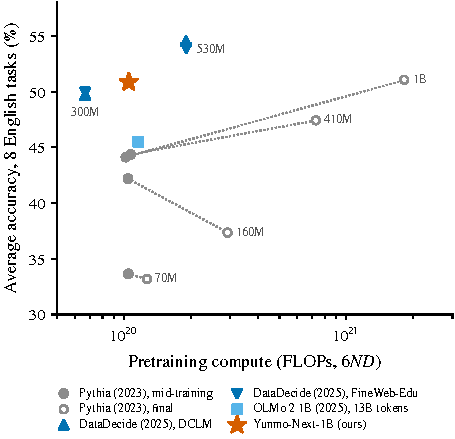
\includegraphics[width=0.55\textwidth]{../figures/compute_scatter.pdf}
  \caption{Average accuracy on eight English tasks against pretraining compute ($6ND$). Filled grey: Pythia at
  \yn{}'s compute; open grey: the same sizes after full training.}
  \label{fig:compute}
\end{figure}

\begin{table}[t]
\centering\small
\caption{Equal-compute comparison. English: average of ARC-Easy, ARC-Challenge, HellaSwag, PIQA, Winogrande,
OpenBookQA, SciQ and LAMBADA.}\label{tab:compute}
\begin{tabular}{@{}lrrr@{}}
\toprule
Model & Compute (FLOPs) & English avg. & XWinograd-zh \\
\midrule
\yn{} & $1.05\times10^{20}$ & 50.9 & 67.5 \\
DataDecide 300M, FineWeb-Edu / DCLM & $0.67\times10^{20}$ & 49.9 / 49.7 & 52.8 / 53.0 \\
DataDecide 530M, FineWeb-Edu / DCLM & $1.90\times10^{20}$ & 53.9 / 54.6 & 52.6 / 53.8 \\
OLMo 2 1B, 13B tokens (mid-training) & $1.16\times10^{20}$ & 45.5 & 51.8 \\
Best Pythia at equal compute (410M) & $1.07\times10^{20}$ & 44.4 & 52.0 \\
Pythia-1B, final & $18.2\times10^{20}$ & 51.1 & 59.1 \\
\bottomrule
\end{tabular}
\end{table}

\yn{} is 0.9--1.2 points above the DataDecide 300M models, which used 64\% of its compute, and 3.1--3.7 points
below the 530M models, which used 181\%; it is highest on SciQ and Winogrande, and behind the 530M models on ARC,
HellaSwag and PIQA. Those models were trained on English only, while about 70\% of our tokens were Chinese or
code. The comparison measures the whole recipe, data included, not the architecture.

\subsection{Cloze formulation and continuous metrics}

Letter-scored multiple choice stays at chance for small models. Following OLMES~\cite{olmes2024} we also score
the text of each answer (cloze form; for TMMLU+ we wrote a cloze variant in which the question is followed by the Chinese
word for ``answer'' and a colon), and following DataDecide~\cite{datadecide2025} we report two continuous metrics: the probability of the correct choice, normalized over
the choices, and the bits per byte of the correct answer text. On TMMLU+ (19,680 items) no model of 1.2B
parameters or fewer is above chance, by accuracy (22.9--25.3\%) or by the normalized probability of the correct
choice (23.1--25.4\%; \yn{} 24.6\%); only the 2B reference is (28.3\% and 27.8\%). \yn{} gives the correct
answer text the lowest bits per byte of these models (1.337, against 1.357 for Qwen3.5-0.8B and 1.394 for
MiniCPM5-1B; 2.1--3.0 for the English-only models), but since it does not prefer the correct choice, this
ranking reflects how well it predicts Traditional Chinese, not knowledge (Figure~\ref{fig:cloze}). On MMLU in
cloze form \yn{} scores 29.3\%, level with the final Pythia-1B (29.6\%) and below the DataDecide 530M models
(30.6--32.5\%).

\begin{figure}[t]
  \centering
  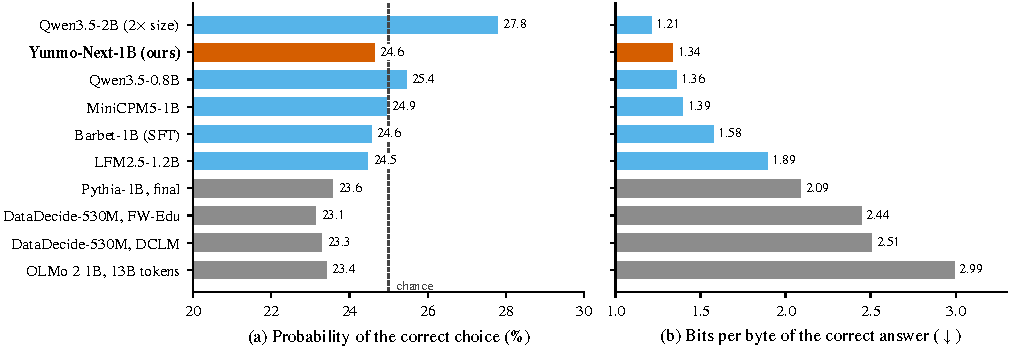
\includegraphics[width=\textwidth]{../figures/tmmluplus_cloze.pdf}
  \caption{TMMLU+ in cloze form. (a) Probability of the correct choice, normalized over the choices. (b) Bits per byte of the correct answer text. Grey: English-only models
  at similar or larger compute.}
  \label{fig:cloze}
\end{figure}

\subsection{Traditional Chinese text}

\paragraph{New Wikipedia articles.} The test set is 3,754 Chinese Wikipedia articles created after 2026-10-01,
after every compared model's release, each cut to its first 2,000 characters. Each model scores each article in
FP32 conditioned on its start token; we report bits per UTF-8 byte, which does not depend on the tokenizer.
\yn{} has the lowest bits per byte (0.918), ahead of MiniCPM5-2B (0.960), Qwen3.5-2B (0.972), Qwen3.5-0.8B
(1.077), MiniCPM5-1B (1.085), Barbet-1B (1.167) and LFM2.5 (1.366). On the Simplified rendering of the same
articles it is level with the 0.8--1B models (1.033 vs.\ 1.030--1.035), so the advantage is specific to
Traditional script.

\paragraph{Overlap.} \yn{} was trained on 0.58B tokens of Chinese Wikipedia, and new articles can reuse older
text. After mapping both sides to one script form with OpenCC, 1.77\% of the test characters are covered by
25-character windows that occur in the Wikipedia build our training data was drawn from (a superset of what the
model saw); 3,077 articles have no covered character. On those articles \yn{} scores 0.932 (others change by at
most 0.004) and remains first, 0.032 ahead of MiniCPM5-2B. With 13-character windows only 568 articles are
uncovered; the order is unchanged on them.

\paragraph{Outside Wikipedia.} Exact overlap does not measure familiarity with encyclopedic style. On three
corpora published by OpenFormosa and absent from our training data, the lead does not carry over
(Figure~\ref{fig:heldout}): \yn{} is level with MiniCPM5-1B on Legislative Yuan transcripts (1.348 vs.\ 1.346),
better on Common Voice sentences (1.755 vs.\ 1.794) and worse on Taiwan localization references (0.560 vs.\
0.534), and Barbet-1B, OpenFormosa's own model, is best on the two spoken-language sets. The accurate summary is
that \yn{} is best on Traditional Chinese encyclopedic text and on par with the strongest 1B models on other
Traditional Chinese text.

\begin{figure}[t]
  \centering
  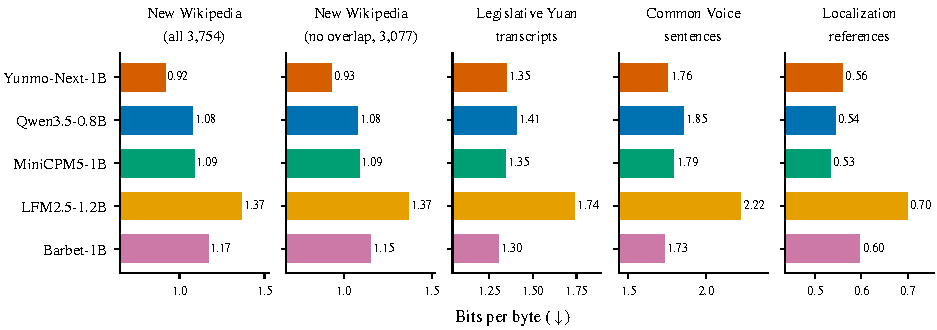
\includegraphics[width=\textwidth]{../figures/heldout_text.pdf}
  \caption{Bits per byte on new Wikipedia articles (all, and those with no 25-character overlap with our
  Wikipedia training data) and on three non-Wikipedia corpora.}
  \label{fig:heldout}
\end{figure}

\subsection{Long context}

On 85 new Wikipedia articles of at least 10,000 characters, \yn{} predicts the first 1,000 characters 0.07--0.15
bits per byte better than Qwen3.5-0.8B and MiniCPM5-1B; from about 4,000 characters they are level, and beyond
about 12,000 characters both are slightly better (Figure~\ref{fig:long}a). Its cache and recurrent state at 32K
tokens is the smallest of the four models (290\,MiB), but its peak memory is the largest (4.5\,GiB) and its
prefill is slower at short context. Synthetic retrieval is weak beyond 8K (multi-query associative recall 40.6\% at 8K, 6.3\% at
16K).

\begin{figure}[t]
  \centering
  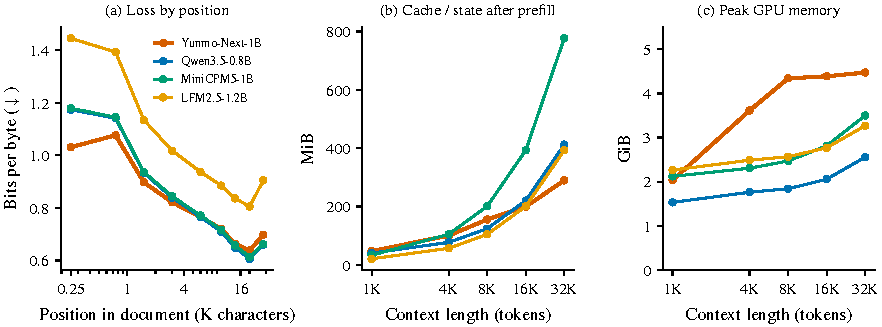
\includegraphics[width=\textwidth]{../figures/long_context.pdf}
  \caption{(a) Bits per byte by position in long new Wikipedia articles. (b) Cache and recurrent state after
  prefill. (c) Peak GPU memory. Batch 1, BF16, RTX 4070 Ti.}
  \label{fig:long}
\end{figure}

\subsection{Instruction-tuned model}

In chat mode with greedy decoding, \yn{}-Instruct scores 44.7 on IFEval, 13.9 on GSM8K, 15.9 on HumanEval, 29.0
on MMLU and 23.0 on TMMLU+ (subsets of 1,140 and 990 items), last among six models on every task; the gap is
smallest on IFEval (7 points behind Qwen3.5-0.8B) and TMMLU+. Reasoning effort works mechanically, but \texttt{medium} and
\texttt{high} score lower than \texttt{none} on every task and \texttt{low} is ahead only on GSM8K, by 1.1
points: the model copies the structure of the distilled
long reasoning traces, including re-checks, without their correctness, consistent with the observation that
small models learn poorly from long chains of thought of much larger teachers~\cite{smallreasoners2025}.

\subsection{Quantized weights}

\begin{figure}[t]
  \centering
  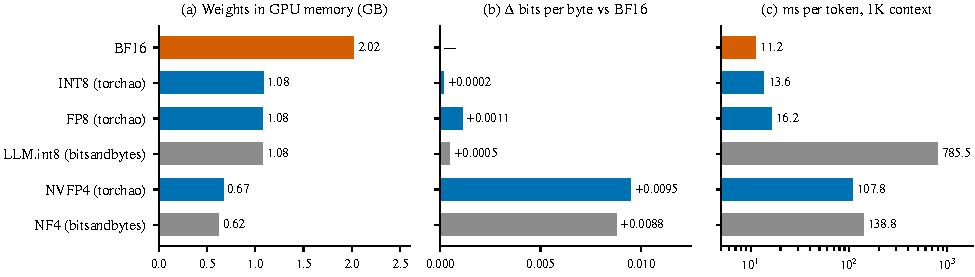
\includegraphics[width=\textwidth]{../figures/quantization.pdf}
  \caption{Quantized weights of the Instruct model: (a) weight memory, (b) loss increase on the new Wikipedia
  articles, (c) decode latency at 1K context, batch 1, RTX 4070 Ti (log scale).}
  \label{fig:quant}
\end{figure}

We release INT8 and FP8 (torchao~\cite{torchao}), NVFP4 and NF4 weights and MLX~\cite{mlx} versions.
Figure~\ref{fig:quant} measures them: 8-bit formats change bits per byte by at most 0.0011 (INT8: $+0.0002$ at
13.6\,ms per token, against 11.2\,ms for BF16), and 4-bit formats by about 0.009, about 1\% of the loss. On the
RTX 4070 Ti, which has no FP4 tensor cores, NVFP4 is dequantized in software and is about ten times slower than
BF16. llama.cpp does not implement this architecture, so there is no GGUF version.

\section{Limitations}

\begin{itemize}
\item \textbf{Knowledge and reasoning.} Letter-scored knowledge benchmarks are at chance for the base model; the
  instruction-tuned model trails 2026 models of similar size on every chat benchmark, and its text is often wrong
  on facts.
\item \textbf{One run.} The route was trained once; intervals reported in the training report are over held-out
  documents, not seeds. Design choices come from short runs at 24 layers.
\item \textbf{Confounded comparisons.} Equal-compute comparisons measure whole recipes; the data, schedule and
  architecture differ together.
\item \textbf{Traditional Chinese evaluation.} The strongest result is on encyclopedic text, the kind the model
  was trained on; the non-Wikipedia sets are short texts and not dated after every model's data.
\item \textbf{Data.} Much of the Chinese text was converted from Simplified script; the share of text originally
  written in Traditional Chinese is not resolved. Some fine-tuning sources restrict commercial use.
\item \textbf{Hardware.} Inference requires a CUDA GPU (or the MLX port); there is no CPU path for the KDA layers.
\end{itemize}

\section{Conclusion}

A 1B hybrid linear-attention model can be pretrained on one consumer GPU for about $10^{20}$ FLOPs. At that
compute its recipe is competitive with annealed English-only references of 2025 while most of its tokens are
Chinese, and it models Traditional Chinese encyclopedic text better than 2026 models trained with
$10^3$--$10^4$ times more compute. Knowledge, reasoning and reliability remain far behind models trained with
more tokens. We release everything needed to reproduce, use and extend the model.

\section*{Artifacts}

Weights, quantized versions and the tokenizer: \url{https://huggingface.co/yuhuanstudio}.
Training, inference and evaluation code: \url{https://github.com/YuhuanStudio/Yunmo-Next}.
Technical reports, evaluation outputs and the sources of every figure: \url{https://github.com/YuhuanStudio/Yunmo-Next-1B}.

\bibliographystyle{plainnat}
\bibliography{references}

\end{document}
